\chapter{.NET platform}

The .NET platform, or any platform implementing the open CLI standard\footnote{\citep{CLIEcma}}, stands on four pillars (\autoref{fig2.1:CLI}). The low level intermediate language CIL, the higher level languages such as C\# and F\# and their compilers to CIL, the base class library known as .NET framework, and - last but not least - the common language runtime, CLR, that actually executes the intermediate code.

\begin{figure}[h]
	\centering	
	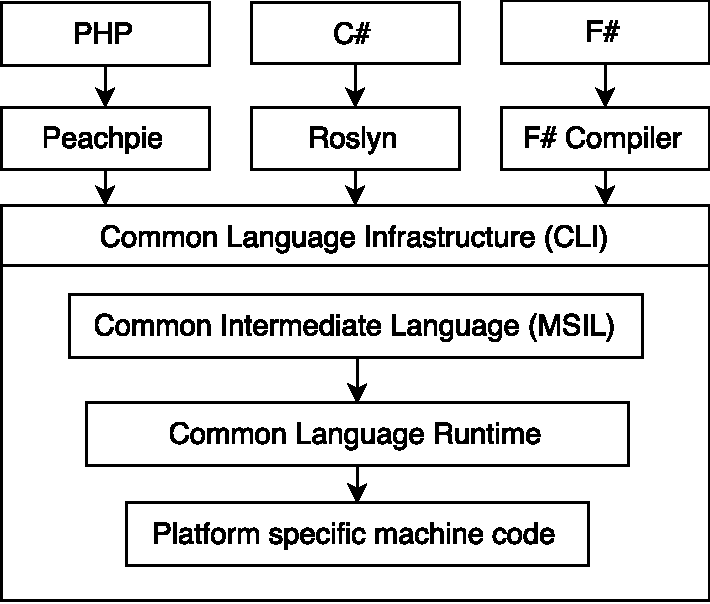
\includegraphics[scale=0.75]{../img/2_1_CLI}	
	\caption{Common language infrastructure.}
	\label{fig2.1:CLI}
\end{figure}

We will talk about the C\# and Visual Basic compiler Roslyn later, but neither the base class library nor the CLR will be covered extensively in this thesis. The common intermediate language, however, will be discussed in detail. 

\section{Common intermediate language}\label{CIL}

CIL is an assembler defined by the common language infrastructure \citep{CLIEcma}\nocite{CSharpEcma} to be a shared basis for all CLI languages (C\#, F\#, IronPython, …) and runtime implementations (.NET, Mono, dotGNU, …). It is platform independent and as such does not natively run on any CPU architecture. Instead, it must be either translated to the target platform’s native code beforehand or - more commonly - executed by a virtual machine such as CLR.

Despite being an assembler, thus inherently low-level, CIL is actually object oriented and so has a deep understanding of reference types. Its instruction set reflects this with means to create new instances, access their members, and so on. The CLI specification also dictates that, by default, the CIL should be memory safe. 

\subsection{Evaluation stack}

CIL is a stack based assembler, therefore without the notion for registers. Instead, it defines a virtual evaluation stack. There are basically two types of instructions in CIL. Firstly, there are memory handling ones that either pop a value from the stack and store it in memory or load a value from memory and push it to the top. Secondly, there are instructions that actually do some processing. These pop a few values from the stack, process them in some way, and then store the result on the top of the stack.

There are a few important things to note about the evaluation stack \citep[Sec. I.12.4]{CLIEcma}. Firstly, all parameters and local variables actually live there. They are not ordinary stack values, though. Their place gets reserved and later cleaned automatically and they are not accessible through the normal push/pop instructions. Instead there are dedicated instructions to work with them.

Secondly, when exiting a function, the stack cannot contain anything but the returned value. Thirdly, there are instructions only to work with its top. There is no way to query all the elements in the stack, get its height, or to completely save or load it to/from memory.

Lastly, while not a rule, the stack is generally used as a store for temporal values instead of proper local variables. For example, an expression $2 + 3 * 5$ (\autoref{list2.1}) would usually result in the load of constants $2$, $3$, and $5$, a multiplication operation $(3 * 5)$ (see \emph{IL\_0009}), at which point the stack would contain $2$ and $15$, and finally a plus operation (see \emph{IL\_000a}) that would leave the stack with $17$ at its top.

\begin{listing}[h]
	\caption{Simple method in C\# and CIL.}
	\label{list2.1}
\begin{minted}{csharp}
public void M(int a) {
  int b = 3;     // IL_0001 & IL_0002
  int c = 5;     // IL_0003 & IL_0004   
  G(a + b * c);  // IL_0005 - IL_000b
}
public int G(int a){/*Something*/}
\end{minted}
\begin{minted}[breaklines=true]{js}
.method public hidebysig instance void M (int32 a) 
cil managed {
  .maxstack 4
  .locals init ([0] int32, [1] int32)
  IL_0000: nop       // Do nothing (No operation)
  IL_0001: ldc.i4.3  // Push 3 onto the stack as int32
  IL_0002: stloc.0   // Pop value from stack to local variable 0
  IL_0003: ldc.i4.5  // Push 5 onto the stack as int32
  IL_0004: stloc.1   // Pop value from stack to local variable 1
  IL_0005: ldarg.0   // Load argument 0 (this) onto the stack
  IL_0006: ldarg.1   // Load argument 1 onto the stack
  IL_0007: ldloc.0   // Load local variable 0 onto stack
  IL_0008: ldloc.1   // Load local variable 1 onto stack
  IL_0009: mul       // Multiply values
  IL_000a: add       // Add two values, returning a new value
  IL_000b: call instance int32 C::G(int32) // Call method indicated on the stack with arguments
  IL_0010: pop       // Pop value (returned by G) from the stack
  IL_0011: ret       // Return from method, possibly with a value
} // end of method C::M
\end{minted}
\end{listing}

All of these mean that you cannot simply pause and save the execution of a method at an arbitrary point with just one or even a few CIL instructions. To completely capture the current state, you not only need to save all the local variables and parameters somewhere off the stack, but you must also do the same for every temporal value that might at that moment live on the stack. And there is no simple way to query what is there. You either need to construct the information in some other way or restrain yourself to saving the state only when the stack is empty.

\subsection{Exception handling}

The last notable thing about CIL is that it has a notion of exceptions and their handling blocks. Try, catch, and finally are all first class citizens in the language and are bound by a number of rules \citep[Sec. I.12.4]{CLIEcma}.

CIL does not permit jumping / branching into any exception handling block\footnote{\citep[Sec. I.12.4.2.8.2.7]{CLIEcma}} unless the source of the jump / branch is within the same block. You can only enter catch and finally regions through the proper exception handling mechanism. And lastly, to leave any of them\footnote{\citep[Sec. I.12.4.2.8.2.8]{CLIEcma}}, you need to do it via a designed instruction that, in case of try and catch blocks, ensures any potential finally region gets run. Therefore, you can neither jump in the middle of a try block nor execute a catch / finally block without throwing a proper exception first.

